\documentclass[11pt]{article}

\usepackage[margin=1in]{geometry}
\usepackage{amsmath}
\usepackage{amssymb}
\usepackage{booktabs}
\usepackage{array}
\usepackage{xcolor}
\usepackage[colorlinks=true,linkcolor=blue!50!black,urlcolor=blue!50!black]{hyperref}

% light-weight code styling
\usepackage{fancyvrb}
\fvset{fontsize=\small,frame=single,framesep=6pt,xleftmargin=4pt}

% figures
\usepackage{tikz}
\usetikzlibrary{calc}
\definecolor{coral}{HTML}{C4441D}
\definecolor{spoke}{HTML}{9C9A92}
\definecolor{hpent}{HTML}{534AB7}

\newcommand{\phigr}{\varphi}
\newcommand{\Hn}[4]{H(#1,#2,#3,#4)}
\newcommand{\Pn}[2]{P(#1,#2)}

\title{\textbf{HafBase}\\[4pt]
\large An Exact Half-Angle Extension of Golden-Ratio Arithmetic\\
\large for Building With Fivefold and Square Corners}
\author{James A. Hinds (Geemo)\\ SpaceStruts Research}
\date{July 2026}

\begin{document}
\maketitle

\begin{abstract}
Golden-ratio arithmetic works with numbers of the form $n + p\phigr$, where $\phigr$ is the
golden ratio and $\phigr^2 = \phigr + 1$. It grids the pentagon exactly and is at home in three
dimensions, where a dodecahedron's vertices are all golden integers. But an upright pentagon and
a square corner cannot share exact Cartesian coordinates: the sine of a pentagon angle,
$\sin 36^\circ$, is simply not expressible as $n + p\phigr$. So the moment you rotate a face onto the
plane to work with it, the exactness breaks.

HafBase fixes this by adding one new number, $\psi = 2\cos 18^\circ$, which cuts the basic
$36^\circ$ step in half to $18^\circ$. Five $18^\circ$ turns then make exactly $90^\circ$.
The extra arithmetic is a single new reduction rule, $\psi^2 = 2 + \phigr$, sitting on top of the golden
$\phigr^2 = \phigr + 1$, and a HafBase number is just four integers,
$\Hn{a}{b}{c}{d} = a + b\phigr + c\psi + d\phigr\psi$ (with real unit coordinates carrying a shared
power-of-two scale). The doubled sine becomes a clean HafBase integer, $2\sin 36^\circ = (\phigr-1)\psi
= \Hn{0}{0}{-1}{1}$. Every calculation reduces
to ordinary golden-ratio arithmetic done twice. This paper builds the whole thing from that one
rule, with the arithmetic shown by worked example at each step, and shows how it gives drift-free
construction where fivefold and square framing meet. The development is procedural throughout: every
rule is stated as a reduction, shown by worked example, and checked by computation, with the field-theory
justification left to whoever wants to reconstruct it from the one reduction rule.
\end{abstract}

\section{The problem, in a picture}

The tiny alga \emph{Braarudosphaera bigelowii} grows a mineral shell shaped like a regular
dodecahedron --- twelve pentagon faces. Each face is carved into five identical four-sided tiles by
spokes running from the face center to the middle of each edge, and every tile has corner angles
$108^\circ$, $90^\circ$, $72^\circ$, $90^\circ$. The two right angles sit where a spoke meets an edge
at its midpoint. Figure~\ref{fig:trig} draws one face, set upright on the XY plane the way you would to
work with it, with the spoke pattern that gives the shell its look.

\begin{figure}[h]
\centering
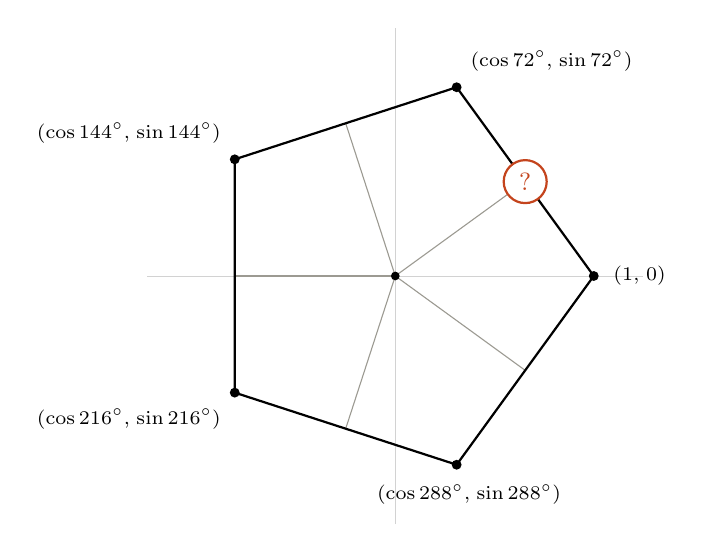
\begin{tikzpicture}[scale=1.05,>=stealth]
  \draw[gray!35,very thin] (-3.0,0)--(3.0,0);
  \draw[gray!35,very thin] (0,-3.0)--(0,3.0);
  \foreach \a in {0,72,144,216,288} \coordinate (V\a) at (\a:2.4);
  \foreach \a in {36,108,180,252,324} \coordinate (M\a) at (\a:1.9416);
  \foreach \a in {36,108,180,252,324} \draw[spoke,thin] (0,0)--(M\a);
  \draw[black,thick] (V0)--(V72)--(V144)--(V216)--(V288)--cycle;
  \fill (0,0) circle (1.5pt);
  \foreach \a in {0,72,144,216,288} \fill (V\a) circle (1.7pt);
  \node[anchor=west]       at ($(V0)+(0.12,0)$)    {$\scriptstyle (1,\;0)$};
  \node[anchor=south west] at ($(V72)+(0.05,0.08)$)  {$\scriptstyle (\cos 72^\circ,\;\sin 72^\circ)$};
  \node[anchor=south east] at ($(V144)+(-0.05,0.08)$){$\scriptstyle (\cos 144^\circ,\;\sin 144^\circ)$};
  \node[anchor=north east] at ($(V216)+(-0.05,-0.08)$){$\scriptstyle (\cos 216^\circ,\;\sin 216^\circ)$};
  \node[anchor=north]      at ($(V288)+(0.15,-0.12)$){$\scriptstyle (\cos 288^\circ,\;\sin 288^\circ)$};
  \fill[white] (M36) circle (0.26);
  \draw[coral,thick] (M36) circle (0.26);
  \node[coral] at (M36) {\small ?};
\end{tikzpicture}
\caption{One face of the \emph{Braarudosphaera} shell, rotated to the XY surface. The five spokes from
the center to the edge midpoints carve the face into its five kite tiles. The ``?'' marks the top-right
edge midpoint --- a $90^\circ$ tile corner, and the point this paper is about. Every $x$-coordinate is a
cosine; every $y$-coordinate is a sine.}
\label{fig:trig}
\end{figure}

Put one vertex at $(1,0)$ and space the other four every $72^\circ$. Nothing in the figure is exotic ---
a calculator hands you all ten numbers. But hold onto the $y$-coordinates. They are about to become the
whole story.

\paragraph{Golden arithmetic, and where it shines.} Golden-ratio arithmetic --- \emph{PhiBase} --- stores
a number as two whole numbers,
\[
P(n,p) = n + p\phigr, \qquad \phigr = \tfrac{1+\sqrt5}{2} \approx 1.618, \qquad \phigr^2 = \phigr + 1,
\]
with $n$ and $p$ always integers and one reduction rule, $\phigr^2 = \phigr + 1$: whenever a $\phigr^2$ turns
up it reduces back to $\phigr + 1$, so multiplication never leaves the whole-number pairs. In three
dimensions this is a triumph. The dodecahedron's twenty vertices are exact golden integers --- the eight
corners $(\pm1,\pm1,\pm1)$ together with the twelve points $(0,\pm\tfrac{1}{\phigr},\pm\phigr)$ and their
rotations --- every coordinate a clean $P(n,p)$, no rounding, no drift. The same encoding carries the
SixPhi construction and the whole solid (as explored on the teaching site,
\href{https://spacestruts.com}{spacestruts.com}). Two integers per coordinate, exact, in space. PhiBase
looks like the answer to everything.

\paragraph{The doubled-cosine convention.} Rotating a shape needs cosines and sines, and one small
convention pays off first. The bare cosine of a pentagon angle is fractional, but \emph{twice} the cosine
is a clean golden whole number:
\[
2\cos 36^\circ = \phigr, \qquad 2\cos 72^\circ = \phigr - 1, \qquad 2\cos 108^\circ = 1 - \phigr,
\qquad 2\cos 144^\circ = -\phigr.
\]
(Check the first: $\cos 36^\circ = 0.809\ldots$ and $\phigr/2 = 0.809\ldots$.) So the golden ratio
\emph{is itself a doubled cosine}, $\phigr = 2\cos 36^\circ$ --- the factor of two is exactly what turns
the fractional $\cos 36^\circ$ into the whole-number $\phigr$ that obeys $\phigr^2 = \phigr + 1$. We carry
doubled cosines throughout, halving only at the very end when a real coordinate needs it. Hold onto that
factor of two; it comes back in the next section.

\paragraph{Until you rotate a face to the XY surface.} Now take one face and rotate it to the XY surface
to work with it in two dimensions --- exactly Figure~\ref{fig:trig}. The vertices that were pure golden in
3-space now carry heights that are sines of pentagon angles, and \emph{those sines are what golden
arithmetic cannot write}. The $x$-coordinates survive the trip --- $2\cos 72^\circ = \phigr - 1$ is
golden --- but $\sin 36^\circ = 0.5878\ldots$ is not $P(n,p)$ for any integers $n,p$; it needs a square
root that $\mathbb{Z}[\phigr]$ does not contain. Every $y$ in Figure~\ref{fig:trig} is a sine, and the
sines are the wall.

That the failure is this specific is the good news, because it locates the cure. PhiBase never broke ---
the solid stays golden. What needs a new number is the \emph{operator that rotates a face to the XY
surface}, and that rotation turns the pentagon's frame through an extra $18^\circ$. So the missing number
should be built from $18^\circ$. The rest of the paper builds it, starting from that one angle.

\section{The one new number}

The trick is to cut the basic $36^\circ$ step in half. Following exactly the doubled-cosine convention
we just used for $\phigr = 2\cos 36^\circ$, we take the doubled cosine of the half-angle:
\[
\boxed{\;\psi = 2\cos 18^\circ \approx 1.9021130326\;}
\]
The factor of two is there for the very same reason it was there for $\phigr$: the bare $\cos 18^\circ$ is
fractional and would drag a denominator of two through every calculation, while the doubled value $\psi$
is a clean whole-number citizen. Where $\phigr$ was the doubled cosine of the pentagon's basic $36^\circ$
turn, $\psi$ is the doubled cosine of \emph{half} that turn. Now find out how $\psi$ behaves when you
square it. Using the standard identity $2\cos^2\theta = 1 + \cos 2\theta$ with $\theta = 18^\circ$:
\[
\psi^2 = 4\cos^2 18^\circ = 2\,(1 + \cos 36^\circ) = 2 + 2\cos 36^\circ = 2 + \phigr.
\]
Check it numerically: $\psi^2 = (1.9021130326)^2 = 3.6180339887\ldots$, and $2 + \phigr = 2 + 1.6180339887 =
3.6180339887\ldots$. They match. So we have found the \textbf{one new reduction rule} to add on top of
$\phigr^2 = \phigr + 1$ --- multiplication uses both:
\[
\boxed{\;\psi^2 = 2 + \phigr\;}
\]
Everything below is bookkeeping on top of this. Where golden arithmetic reduces $\phigr^2$ back to
$\phigr + 1$, HafBase also reduces $\psi^2$ back to $2 + \phigr$. Two reduction rules, and nothing else.

\section{HafBase numbers are four integers}

A HafBase number is built from four integers $a, b, c, d$:
\[
\Hn{a}{b}{c}{d} \;=\; a + b\phigr + c\psi + d\phigr\psi.
\]
It helps to read it as two golden numbers stacked. Group the plain part and the $\psi$ part:
\[
\Hn{a}{b}{c}{d} \;=\; \underbrace{(a + b\phigr)}_{\text{ground floor } P_0} \;+\;
\underbrace{(c + d\phigr)}_{\psi\text{-floor } P_1}\,\psi .
\]
So a HafBase number is a \emph{ground floor} $P_0 = \Pn{a}{b}$ and an upstairs \emph{$\psi$-floor}
$P_1 = \Pn{c}{d}$, each an ordinary golden number. Every operation we define is just golden
arithmetic run on these two floors.

Two special values are worth memorizing right away:
\[
\phigr = \Hn{0}{1}{0}{0}, \qquad \psi = \Hn{0}{0}{1}{0}.
\]
And any old golden number $\Pn{a}{b}$ becomes the HafBase number $\Hn{a}{b}{0}{0}$ --- you just
pad the two new slots with zero. So HafBase contains all of golden arithmetic, untouched, sitting
in the ``$\psi$-floor is empty'' numbers.

\section{Coordinates carry a scale}
\label{sec:scale}

One honest caveat before we compute. The four-integer tuples represent \emph{doubled} coordinates ---
values like $2\cos 18^\circ = \psi$ and $2\sin 36^\circ = (\phigr-1)\psi$. The real unit-length
coordinates themselves carry a factor of one-half, and the pentagon's edge midpoint carries a
factor of one-quarter:
\[
\cos 18^\circ = \tfrac12\Hn{0}{0}{1}{0}, \qquad
\sin 36^\circ = \tfrac12\Hn{0}{0}{-1}{1}, \qquad
M = \left(\tfrac14\Hn{1}{1}{0}{0},\ \tfrac14\Hn{0}{0}{1}{0}\right).
\]
Every such denominator is a power of two. So the exact coordinate system is the four-integer ring with
powers of two allowed downstairs --- a \emph{scaled} HafBase value,
\[
H_s(a,b,c,d) = 2^{-s}\,\Hn{a}{b}{c}{d},
\]
stored as the four integers plus one scale exponent $s$, which a whole vector or matrix can share.
Multiplication just adds the exponents; whenever all four coefficients come out even, you divide them
by two and drop $s$ by one to normalize. The integer arithmetic of the following sections is the core;
the scale exponent rides along on top and never complicates a reduction. When we say a doubled cosine ``is''
a HafBase integer, that integer is the tuple at $s = 1$.

\section{Adding: just line up the slots}

Addition could not be simpler --- add matching slots:
\[
\Hn{a}{b}{c}{d} + \Hn{e}{f}{g}{h} = \Hn{a+e}{b+f}{c+g}{d+h}.
\]
For example, $(1 + \psi) + (\phigr + \psi) = \Hn{1}{0}{1}{0} + \Hn{0}{1}{1}{0} = \Hn{1}{1}{2}{0}
= 1 + \phigr + 2\psi$. No reduction is ever needed for addition, because adding never produces a
$\psi^2$.

\section{Multiplying: expand, then reduce}

Multiplication is where the rule $\psi^2 = 2 + \phigr$ earns its keep. Write the two numbers as
floors, $X = P_0 + P_1\psi$ and $Y = Q_0 + Q_1\psi$, and multiply them out like any two binomials:
\[
XY = P_0 Q_0 + (P_0 Q_1 + P_1 Q_0)\psi + P_1 Q_1 \psi^2 .
\]
The last term has a $\psi^2$ in it. Reduce it using the rule, $\psi^2 = 2 + \phigr$:
\[
\boxed{\;XY = \underbrace{\big(P_0 Q_0 + (2+\phigr)\,P_1 Q_1\big)}_{\text{new ground floor}}
\;+\; \underbrace{\big(P_0 Q_1 + P_1 Q_0\big)}_{\text{new }\psi\text{-floor}}\,\psi\;}
\]
That is four golden multiplications ($P_0Q_0$, $P_1Q_1$, $P_0Q_1$, $P_1Q_0$), one multiplication by
the fixed number $2 + \phigr = \Pn{2}{1}$, and some adding. Nothing leaves golden arithmetic.

\paragraph{Worked example.} Let us square $1 + \psi$, i.e. compute $\Hn{1}{0}{1}{0}\times\Hn{1}{0}{1}{0}$.
Here $P_0 = Q_0 = \Pn{1}{0} = 1$ and $P_1 = Q_1 = \Pn{1}{0} = 1$ (the ``$1$'' in the $\psi$-floor
means one copy of $\psi$).
\begin{itemize}
\item Ground pieces: $P_0Q_0 = 1$, and $P_1Q_1 = 1$.
\item Reduce the $\psi^2$ piece: $(2+\phigr)\cdot 1 = 2 + \phigr$.
\item New ground floor: $1 + (2 + \phigr) = 3 + \phigr$.
\item $\psi$-floor pieces: $P_0Q_1 + P_1Q_0 = 1 + 1 = 2$, so the new $\psi$-floor is $2\psi$.
\end{itemize}
Result: $(1+\psi)^2 = 3 + \phigr + 2\psi = \Hn{3}{1}{2}{0}$.

Sanity check with decimals: $(1 + 1.9021)^2 = 2.9021^2 = 8.4224$, and
$3 + 1.6180 + 2(1.9021) = 3 + 1.6180 + 3.8042 = 8.4224$. It matches exactly. In code
(Section~\ref{sec:verify}), \verb|mulH [1,0,1,0], [1,0,1,0]| returns \verb|[3,1,2,0]|.

The only new helper you need beyond a golden-arithmetic library is ``multiply a golden number by
$\psi^2$,'' which is just multiply-by-$\Pn{2}{1}$:
\[
\mathrm{fold}\big(\Pn{x}{y}\big) = \Pn{x}{y}\cdot\Pn{2}{1} = \Pn{2x + y}{\,x + 3y}.
\]

\section{The norm: a whole-number magnitude}

Golden arithmetic comes with a \emph{norm} --- a single whole number that measures a golden quantity's
magnitude and tells you whether it can be divided out cleanly. For $\Pn{n}{p}$ it is
\[
N\big(\Pn{n}{p}\big) = n^2 + np - p^2,
\]
always an ordinary integer. (It is the number multiplied by its golden mirror image $n + p(1-\phigr)$,
which is why the result lands on a plain integer.) HafBase has the same idea in two steps. First collapse
the $\psi$-floor down to a single golden number,
\[
(\text{relative norm of } X) = P_0^2 - (2 + \phigr)\,P_1^2 ,
\]
then take the golden norm of that to reach a plain whole number. The norm is what you use to test whether
a HafBase number is reversible --- a norm of $\pm 1$ means it is a \emph{unit}, so division by it is exact
--- and as an all-integer exactness check.

\paragraph{Worked example.} The norm of $\psi = \Hn{0}{0}{1}{0}$: here $P_0 = \Pn{0}{0} = 0$ and
$P_1 = \Pn{1}{0} = 1$, so the relative norm is $0 - (2+\phigr)\cdot 1 = -(2 + \phigr) = \Pn{-2}{-1}$.
Its golden norm is $(-2)^2 + (-2)(-1) - (-1)^2 = 4 + 2 - 1 = 5$. So $\psi$ has norm $5$ --- not $\pm1$,
so $\psi$ is not reversible on its own. By contrast $\phigr$ is a unit: its HafBase norm is $+1$ (its
PhiBase norm is $-1$, and the HafBase norm squares that, since $\phigr$ embeds as a golden number), and
indeed $1/\phigr = \phigr - 1$ exactly. The golden ``scale ladder'' of powers of $\phigr$ therefore
survives inside HafBase untouched, and we keep it as the designated scale ladder. That $\psi$ itself is
not a unit does not mean the enlarged ring gains no new units --- it does, mixed ones like $1 + \psi$
(with norm $1$) --- but the construction here deliberately measures scale in powers of $\phigr$ and uses
$\psi$ only for direction. In code the norm of $\psi$ is \verb|normH [0,0,1,0]|, returning \verb|5|.

\section{Every $18^\circ$ direction now has exact coordinates}

Here is the payoff that makes the pentagon and the square corner get along. The key fact is a
one-line calculation.

\paragraph{The sine, found.} Claim: $2\cos 54^\circ = (\phigr - 1)\psi$, which means
$\sin 36^\circ = \tfrac{1}{2}(\phigr-1)\psi$ (since $\sin 36^\circ = \cos 54^\circ$). To check it,
square both sides. Left: $(2\cos 54^\circ)^2 = 2(1 + \cos 108^\circ) = 2 + (1 - \phigr) = 3 - \phigr$
(using $2\cos 108^\circ = 1 - \phigr$). Right: $\big((\phigr-1)\psi\big)^2 = (\phigr-1)^2\psi^2
= (2 - \phigr)(2 + \phigr) = 4 - \phigr^2 = 4 - (\phigr + 1) = 3 - \phigr$. Same value, and both are
positive, so they are equal.

That is the whole ballgame. The number $\sin 36^\circ$ --- the exact thing golden arithmetic could
not write --- is now within reach: its \emph{double} is a clean HafBase integer,
\[
2\sin 36^\circ = (\phigr-1)\psi = \Hn{0}{0}{-1}{1}, \qquad\text{so}\qquad \sin 36^\circ = \tfrac12\,\Hn{0}{0}{-1}{1},
\]
exactly, with the factor $\tfrac12$ carried in the coordinate scale (Section~\ref{sec:scale}). And once
one odd angle is inside, the
whole $18^\circ$ family is. Using the ``store the doubled cosine'' convention (which keeps
everything as whole numbers instead of halves), the complete angle table is:

\begin{center}
\begin{tabular}{c c l}
\toprule
angle $\theta$ & $2\cos\theta$ & as HafBase \\
\midrule
$18^\circ$  & $\psi$            & $\Hn{0}{0}{1}{0}$ \\
$36^\circ$  & $\phigr$          & $\Hn{0}{1}{0}{0}$ \\
$54^\circ$  & $(\phigr-1)\psi$  & $\Hn{0}{0}{-1}{1}$ \\
$72^\circ$  & $\phigr - 1$      & $\Hn{-1}{1}{0}{0}$ \\
$90^\circ$  & $0$               & $\Hn{0}{0}{0}{0}$ \\
$108^\circ$ & $1 - \phigr$      & $\Hn{1}{-1}{0}{0}$ \\
$126^\circ$ & $-(\phigr-1)\psi$ & $\Hn{0}{0}{1}{-1}$ \\
$144^\circ$ & $-\phigr$         & $\Hn{0}{-1}{0}{0}$ \\
$162^\circ$ & $-\psi$           & $\Hn{0}{0}{-1}{0}$ \\
\bottomrule
\end{tabular}
\end{center}

Notice the pattern, and read it carefully --- this is a table of \emph{cosines}, not of directions.
The multiples of $36^\circ$ ($36, 72, 108, 144$) have an empty $\psi$-floor: their doubled cosines are
golden. The odd multiples ($18, 54, 126, 162$) use the $\psi$-floor. And the right angle, $90^\circ$,
is the single row that is exactly zero: $2\cos 90^\circ = 0$, needing neither $\phigr$ nor $\psi$.

But a full direction needs a cosine \emph{and} a sine, and the sines tell a different story. Even at a
multiple of $36^\circ$, the sine carries $\psi$: the $36^\circ$ direction is
$2(\cos 36^\circ, \sin 36^\circ) = (\Hn{0}{1}{0}{0},\, \Hn{0}{0}{-1}{1})$ --- golden across, but
$\psi$-bearing up. So except along the square axes, an exact Cartesian direction vector normally uses one
golden coordinate and one that carries $\psi$. This is exactly the ``rotate a face onto the plane and the
heights become sines'' wall from Section~1, now written in the new arithmetic: the $\psi$-floor is where
those sines live.

The practical meaning: in HafBase you can work in plain $x,y$ coordinates and stay exact for every
$18^\circ$ direction, because the one number that used to force slanted coordinates, $\sin 36^\circ$,
is now available. Pentagon axes and square axes live together in one exact system.

Figure~\ref{fig:psi} is Figure~\ref{fig:trig} redrawn with $\psi$ in hand. The heights that were bare
sines are now writable: the $\sin 72^\circ$ height is $\psi/2$, and the $\sin 36^\circ$ height is
$(\phigr-1)\psi/2$. Same face, same spokes --- but the wall is gone, and even the ``?'' midpoint has an
exact name.

\begin{figure}[h]
\centering
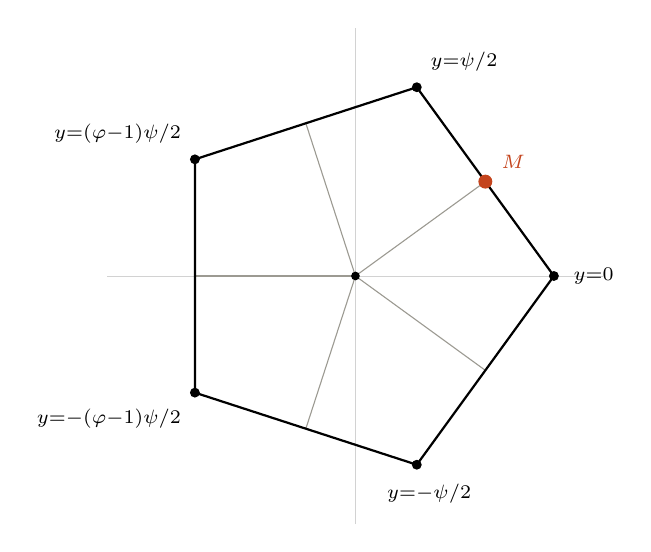
\begin{tikzpicture}[scale=1.05,>=stealth]
  \draw[gray!35,very thin] (-3.0,0)--(3.0,0);
  \draw[gray!35,very thin] (0,-3.0)--(0,3.0);
  \foreach \a in {0,72,144,216,288} \coordinate (V\a) at (\a:2.4);
  \foreach \a in {36,108,180,252,324} \coordinate (M\a) at (\a:1.9416);
  \foreach \a in {36,108,180,252,324} \draw[spoke,thin] (0,0)--(M\a);
  \draw[black,thick] (V0)--(V72)--(V144)--(V216)--(V288)--cycle;
  \fill (0,0) circle (1.5pt);
  \foreach \a in {0,72,144,216,288} \fill (V\a) circle (1.7pt);
  \node[anchor=west]       at ($(V0)+(0.12,0)$)     {$\scriptstyle y=0$};
  \node[anchor=south west] at ($(V72)+(0.05,0.08)$)   {$\scriptstyle y=\psi/2$};
  \node[anchor=south east] at ($(V144)+(-0.05,0.08)$) {$\scriptstyle y=(\phigr-1)\psi/2$};
  \node[anchor=north east] at ($(V216)+(-0.05,-0.08)$){$\scriptstyle y=-(\phigr-1)\psi/2$};
  \node[anchor=north]      at ($(V288)+(0.15,-0.12)$) {$\scriptstyle y=-\psi/2$};
  \fill[coral] (M36) circle (2.4pt);
  \node[coral,anchor=south west] at ($(M36)+(0.08,0.04)$) {$\scriptstyle M$};
\end{tikzpicture}
\caption{The same face, once $\psi = 2\cos 18^\circ$ is in hand. Every $x$-coordinate is the golden cosine
it always was; every $y$-coordinate --- a bare sine in Figure~\ref{fig:trig} --- is now a clean multiple
of $\psi$. The midpoint $M$ (the former ``?'') is exact too: clearing its two halves, $4M =
(\Hn{1}{1}{0}{0}, \Hn{0}{0}{1}{0})$ --- that is, $x = \phigr^2$ and $y = \psi$.}
\label{fig:psi}
\end{figure}

\section{Turning by $18^\circ$, and why five turns make a right angle}

A turn by angle $\theta$ in the plane is the matrix
$\left[\begin{smallmatrix}\cos\theta & -\sin\theta\\ \sin\theta & \cos\theta\end{smallmatrix}\right]$.
For $18^\circ$, use $\cos 18^\circ = \psi/2$ and $\sin 18^\circ = \cos 72^\circ = (\phigr-1)/2$. To keep
whole numbers, carry the doubled matrix $2R_{18}$, whose entries are HafBase integers straight from
the table:
\[
2R_{18} =
\begin{pmatrix} \psi & 1-\phigr \\ \phigr - 1 & \psi \end{pmatrix}
=
\begin{pmatrix} \Hn{0}{0}{1}{0} & \Hn{1}{-1}{0}{0} \\[2pt] \Hn{-1}{1}{0}{0} & \Hn{0}{0}{1}{0} \end{pmatrix}.
\]
Its determinant is $\psi^2 + (\phigr - 1)^2 = (2 + \phigr) + (2 - \phigr) = 4$, so $R_{18}$ itself has
determinant $1$ --- it really is a rotation, exactly.

Now turn five times. Five $18^\circ$ turns should give one $90^\circ$ turn, and in HafBase this comes
out perfectly clean:
\[
R_{18}^{\,5} = R_{90} = \begin{pmatrix} 0 & -1 \\ 1 & 0 \end{pmatrix} \quad\text{exactly.}
\]
We are carrying the \emph{doubled} matrix $2R_{18}$ to stay on whole numbers, and each of the five factors
brings a factor of two along, so the doubled statement carries $2^5 = 32$ out front:
\[
(2R_{18})^5 = 2^5\,R_{90} = 32\,R_{90}
= \begin{pmatrix} \Hn{0}{0}{0}{0} & \Hn{-32}{0}{0}{0} \\[3pt] \Hn{32}{0}{0}{0} & \Hn{0}{0}{0}{0} \end{pmatrix}.
\]
The $32$ is only that bookkeeping factor $2^5$; divide it out and you are left with $R_{18}^5 = R_{90}$
exactly. The real content is not that five $18^\circ$ turns make $90^\circ$ --- that is just geometry ---
but that in HafBase \emph{every step of the way stays inside the system} and the $\psi$-floor cancels out
completely at the fifth turn, leaving whole numbers with zero error. This is the check every
implementation must pass (Section~\ref{sec:verify}).

Repeating $R_{18}$ walks through all twenty directions spaced $18^\circ$ apart. The even steps (every
$36^\circ$) have golden \emph{cosines}; the odd steps carry $\psi$ in the cosine too. But as a full
rotation \emph{matrix} even the $36^\circ$ turn already carries $\psi$ in its sine entries --- squaring
the doubled matrix gives $(2R_{18})^2 = 4R_{36}$ with $\psi$-bearing off-diagonals --- so the pentagon
rotations were never wholly golden to begin with. Worth naming what HafBase actually supplies: the right
angle $R_{90} = \left(\begin{smallmatrix}0&-1\\1&0\end{smallmatrix}\right)$ was always available over the
plain integers. What was missing was the sine data of the pentagon angles and the exact $18^\circ$
relative orientation that locks the fivefold and square angle grids together. That is the new content,
and $R_{18}$ is where it lives.

\section{Building things with HafBase}

The features above are exactly what a construction or assembly system wants.

\paragraph{Fivefold and square in one coordinate type.} Because one system holds both the pentagon
turns and the right angle, a design that mixes them --- a fivefold dome on a rectangular base,
pentagon bracing on a square frame --- is written in a single coordinate type. There is no conversion
sitting between the fivefold part and the square part, so no rounding creeps in where they join. That
join is exactly where floating-point pipelines accumulate error: every handoff between a fivefold
subassembly and a square world-frame rounds a little. In HafBase the handoff is an exact identity.

\paragraph{Yes/no questions instead of ``close enough''.} With the angle table as a fixed lookup,
the basic questions of assembly become exact whole-number tests. ``Are these two struts
perpendicular?'' is ``is the doubled dot product equal to $\Hn{0}{0}{0}{0}$?'' --- and equality and
zero tests like it reduce cleanly to the norm: $N_H(X) = 0$ exactly when $X = 0$. Orientation questions
--- left-of, inside --- are different: they need the exact \emph{sign} of the value $X$ in the intended
real embedding, and that is \emph{not} the sign of the algebraic norm (the norm is a signed quantity of
its own, e.g.\ $N_H(1 + \phigr\psi) = -4$ though $1 + \phigr\psi > 0$). The exact sign is still found
without floating point: split $X = P_0 + P_1\psi$, take the exact signs of the two golden floors $P_0$
and $P_1$, and when they disagree, decide the contest by sign-testing $P_0^2 - (2+\phigr)P_1^2$ in
PhiBase. Either way the assembler never asks whether an angle is \emph{close} to a right angle; it asks
whether a whole number is zero, or which of two whole numbers is larger.

\paragraph{The motivating midpoint, computed.} Return to the \emph{Braarudosphaera} edge midpoint ---
the $90^\circ$ corner of that half-tile. Place the pentagon with its center at the origin and one
vertex out along the $x$-axis at distance $1$. The midpoint of an edge sits in the direction
$36^\circ$ (halfway between two vertices $72^\circ$ apart) at a distance equal to the pentagon's
apothem. Two facts make it exact:
\begin{itemize}
\item The \emph{direction} $36^\circ$ has exact coordinates from the table --- and its $y$-part is
built from $\psi$, the new number. A plain rotation only ever gives you a direction, though: it lands
you on the outer circle at distance $1$, not on the midpoint inside.
\item The \emph{distance} to the edge midpoint is the apothem, which equals $\cos 36^\circ = \phigr/2$
--- a pure golden number. So you reach the midpoint by scaling the unit direction by $\phigr/2$.
\end{itemize}
Direction (needs $\psi$) times length (pure $\phigr$) gives the point. Carrying it out and clearing
the fractions by the doubling convention (applied twice, once for the direction's half and once for
the midpoint's half), the midpoint's coordinates times $4$ are
\[
x\text{-coordinate}\times 4 = \Hn{1}{1}{0}{0}, \qquad y\text{-coordinate}\times 4 = \Hn{0}{0}{1}{0}.
\]
Both are exact HafBase whole-number tuples, with the ``$\div 4$'' carried in the scale, never inside
a coordinate. The right angle at that point is then confirmed by a single dot product equal to
$\Hn{0}{0}{0}{0}$. The geometry that motivated this paper is now carried at the same exactness as the
pentagon's own corners.

Figure~\ref{fig:overlay} shows why the $18^\circ$ resolution is exactly what the midpoint needed. Overlay
a second pentagon of the \emph{same size}, turned $36^\circ$: its vertices point in the edge-midpoint
directions of the first, and the two together make the ten-point decagram. The midpoint $M$ sits on the
spoke to a turned-pentagon vertex --- reachable only once the frame can turn in $18^\circ$ steps.

\begin{figure}[h]
\centering
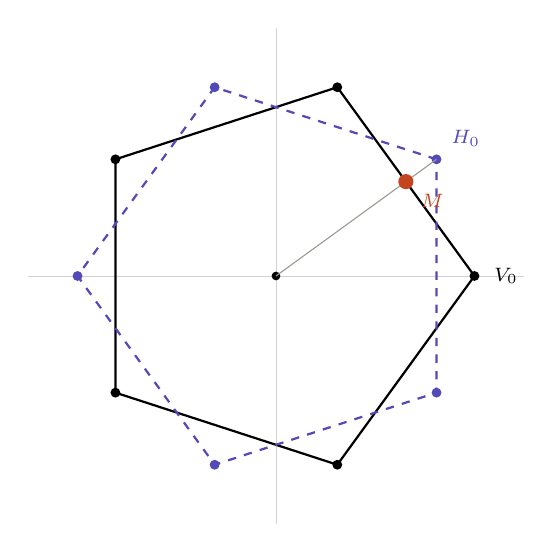
\begin{tikzpicture}[scale=1.05,>=stealth]
  \draw[gray!35,very thin] (-3.0,0)--(3.0,0);
  \draw[gray!35,very thin] (0,-3.0)--(0,3.0);
  \foreach \a in {0,72,144,216,288} \coordinate (V\a) at (\a:2.4);
  \foreach \a in {36,108,180,252,324} \coordinate (H\a) at (\a:2.4);
  \coordinate (M36) at (36:1.9416);
  \draw[black,thick] (V0)--(V72)--(V144)--(V216)--(V288)--cycle;
  \draw[hpent,thick,dashed] (H36)--(H108)--(H180)--(H252)--(H324)--cycle;
  \fill (0,0) circle (1.5pt);
  \foreach \a in {0,72,144,216,288} \fill (V\a) circle (1.7pt);
  \foreach \a in {36,108,180,252,324} \fill[hpent] (H\a) circle (1.7pt);
  \draw[spoke,thin] (0,0)--(H36);
  \fill[coral] (M36) circle (2.6pt);
  \node[anchor=west]       at ($(V0)+(0.12,0)$)  {$\scriptstyle V_0$};
  \node[hpent,anchor=south west] at ($(H36)+(0.06,0.04)$) {$\scriptstyle H_0$};
  \node[coral,anchor=north west] at ($(M36)+(0.06,-0.04)$) {$\scriptstyle M$};
\end{tikzpicture}
\caption{The $P$ pentagon (solid) and a same-size $H$ pentagon turned $36^\circ$ (dashed), forming the
ten-point decagram. The turned vertex $H_0$ points along the same spoke as the edge midpoint $M$, at full
radius; $M$ lies at the apothem distance $\phigr/2$ along that spoke. In doubled Cartesian coordinates
the $P$ vertices read $x$ in PhiBase, $y$ carrying $\psi$; the midpoint is $4M = (\Hn{1}{1}{0}{0},
\Hn{0}{0}{1}{0})$.}
\label{fig:overlay}
\end{figure}

\paragraph{Scale versus direction stay separate.} The powers of $\phigr$ still answer ``how big''
(and $\phigr$ is still reversible, so the golden scale ladder is intact), while $\psi$ answers
``which way,'' at twice the angular resolution. The two never interfere.

\section{Checking an implementation}
\label{sec:verify}

Reuse a tested golden-arithmetic core (add, multiply, norm) and add only the thin HafBase layer.
Each check below is an exact whole-number assertion.

\begin{enumerate}
\item \textbf{Reduction rule.} $\psi\times\psi = \Hn{2}{1}{0}{0}$.
\item \textbf{Embedding.} $\phigr\times\psi = \Hn{0}{0}{0}{1}$, and every golden $\Pn{a}{b}$ round-trips
as $\Hn{a}{b}{0}{0}$.
\item \textbf{Sine.} $\Hn{0}{0}{-1}{1}$ evaluates to $2\sin 36^\circ = 1.1756\ldots$ on a calculator.
\item \textbf{Norm.} The norm of $\psi$ is $5$ (Section~6).
\item \textbf{Closure.} $(2R_{18})^5$ equals $32\,R_{90}$ as a whole-number matrix.
\end{enumerate}

A minimal reference core in CoffeeScript, storing a golden number $\Pn{n}{p}$ as the integer pair
\verb|[n, p]| and a HafBase number $\Hn{a}{b}{c}{d}$ as the integer tuple \verb|[a, b, c, d]|, and
threading the single reduction constant $\Pn{2}{1}$:

\begin{Verbatim}
# Golden core.  A golden number P(n,p) = n + p*phi is the integer pair [n, p],
# with the reduction rule phi^2 = phi + 1.
addPB  = (x, y) -> [x[0] + y[0], x[1] + y[1]]
mulPB  = (x, y) ->
  [a, b] = x
  [c, d] = y
  [a*c + b*d, a*d + b*c + b*d]
normPB = (x) -> x[0]*x[0] + x[0]*x[1] - x[1]*x[1]   # n^2 + n p - p^2

# HafBase.  H(a,b,c,d) = P0 + P1*psi is the integer 4-tuple [a, b, c, d],
# with P0 = [a, b], P1 = [c, d], and the reduction rule psi^2 = 2 + phi.
addH = (X, Y) -> (X[i] + Y[i] for i in [0..3])
fold = (P)    -> mulPB(P, [2, 1])   # multiply by psi^2

mulH = (X, Y) ->
  [P0, P1] = [[X[0], X[1]], [X[2], X[3]]]
  [Q0, Q1] = [[Y[0], Y[1]], [Y[2], Y[3]]]
  ground = addPB(mulPB(P0, Q0), fold(mulPB(P1, Q1)))   # P0Q0 + (2+phi)P1Q1
  psiFloor = addPB(mulPB(P0, Q1), mulPB(P1, Q0))   # P0Q1 + P1Q0
  [ground[0], ground[1], psiFloor[0], psiFloor[1]]

normH = (X) ->               # collapse, then norm
  [P0, P1] = [[X[0], X[1]], [X[2], X[3]]]
  A = mulPB(P0, P0)
  B = fold(mulPB(P1, P1))
  normPB([A[0] - B[0], A[1] - B[1]])

# The acceptance checks (each an exact whole-number result):
mulH([0,0,1,0], [0,0,1,0])   # => [2,1,0,0]  reduce
mulH([0,1,0,0], [0,0,1,0])   # => [0,0,0,1]  phi*psi
mulH([1,0,1,0], [1,0,1,0])   # => [3,1,2,0]  square
normH([0,0,1,0])             # => 5  norm of psi
\end{Verbatim}

These all return exactly the values shown.

\section{Wrap-up}

HafBase is the smallest exact extension of golden-ratio arithmetic in which the pentagon and the
right angle can both be written down at once. A HafBase number is four integers, $\Hn{a}{b}{c}{d}$,
read as two golden numbers stacked over the new number $\psi = 2\cos 18^\circ$. All arithmetic runs
on golden arithmetic plus the one new reduction rule $\psi^2 = 2 + \phigr$. The reward: every $18^\circ$
direction gets exact coordinates, $\sin 36^\circ$ becomes exactly representable (as the half-scaled
integer $\tfrac12\Hn{0}{0}{-1}{1}$), ordinary $x,y$
coordinates become exact for pentagon geometry, and five $18^\circ$ turns close onto a right angle
with zero error. For building things that mix fivefold and square framing, that means one exact
coordinate type across the seam, yes/no geometric tests instead of tolerances, and drift-free closure
through both pentagon and right angles.

\clearpage
\section{Directions for further work}

HafBase closes the plane. Three threads lead out from it, each a construction rather than a proof.

\paragraph{Into three dimensions.} The dodecahedron's vertices already carry golden coordinates, and
HafBase adds exact $18^\circ$ rotations and exact apothem directions \emph{within} each face. The open
task is to stitch the in-face HafBase directions to the vertex lattice across all twelve faces so that a
path crossing from one face to the next stays exact --- an all-integer atlas for the whole solid, with no
drift at the face seams. This is the natural next build for the \emph{Braarudosphaera} geometry that
motivated the paper.

\paragraph{Exact predicates as a fixed table.} The angle palette of Section~7 is already a lookup table;
the same idea extends to the other primitives an assembler needs --- perpendicular, parallel, left-of,
inside. Equality and perpendicularity reduce to the integer test $N_H(X) = 0$; orientation primitives
reduce to the exact sign of $X$ in the real embedding (found in PhiBase, not from the norm's sign, as in
Section~9). Compiling these into a single fixed table of
whole-number tests would give a drift-free geometry kernel that never asks whether an angle is
\emph{close} to a right angle, only whether an integer is zero or which of two is larger.

\paragraph{Real rotations, without imaginary numbers.} One might expect that marrying fivefold and
square symmetry would force complex numbers --- a rotation written as multiplication by $e^{i\theta}$
drags in $i$. It does not, and the reason is worth a note for anyone extending this: planar rotations are
real $2\times2$ matrices needing only $\cos\theta$ and $\sin\theta$, and for every multiple of $18^\circ$
those already sit in the HafBase table. Whether wider symmetry mixtures (say, adding a third symmetry family)
can be kept inside real whole-number arithmetic the same way is an open and useful question.

\end{document}
